% !TeX spellcheck = en_US
% !TEX TS-program = pdflatex
% !TEX encoding = IsoLatin

%% Version 4x3 und 16x9  2.2 02.01.2014

%Based on ETH official latex template
%Modified for ASL by Alvaro Estandia (09.02.2015) (ealvaro@student.ethz.ch)

% ==== wrapper class ==========================================================
\documentclass[% wrapper-class ETHpres option inspite of aspectratio for beamer-classe
    fourtothree=true, % true (default) -- 4:3-format, false -- 16:9-format
    DepLogo=true     % true -- use deplogo_13.pdf, false (default) 
                      %         do not use deplogo_13.pdf for footer
    ]{ETHpres}

% ==== misc: you may use or not ===============================================
%\usepackage{graphicx}   % for including figures
%%\graphicspath{{pictures/}}
%\usepackage{tabularx}   % for special table environment (tabularx-table)
%\usepackage{booktabs}   % for table layout
%\usepackage{natbib}     % for bibliography with astron-style
%\bibliographystyle{astron}
%\usepackage{siunitx}    % to use for international units in the real world
%\usepackage[
%    colorlinks=true, linkcolor=white, urlcolor=white, % this is special for this presentation here to get the toc in white
%    hypertexnames=false,% for correct links (duplicate-error solution)
%	setpagesize=false,  % necessary in order to not change text-/paperformat for the document
%	pdfborder={0 0 0},  % removes border around links
%	pdfpagemode=FullScreen,% open pdf in full screen mode
%    pdfstartview=Fit    % fit page to pdf viewer
%]{hyperref}% all links stay black and are thus invisible

%----- My Packages
\titlespacing{\section}{0pt}{-25pt}{0pt}
\titlespacing{\subsubsection}{0pt}{5pt}{0pt}

\usepackage{amsmath}
\usepackage{caption}
\usepackage{comment}
\usepackage[makeroom]{cancel}


\setitemize{noitemsep,topsep=0pt,parsep=0pt,partopsep=0pt}

%\usepackage{soul} Highligh text \hl{Some Text}
\usepackage{media9} %Add videos

%ASL Packages
\usepackage[numbers]{natbib}
\usepackage{enumitem}
\usepackage{units}

\usepackage{isomath}
\renewcommand{\vec}{\vectorsym}
\newcommand{\mat}{\matrixsym}

% Tikz drawings
\usepackage{tikz}
\usetikzlibrary{calc}

% ==== language ================================================================
\usepackage[latin1]{inputenc}
%\usepackage[utf8]{inputenc}
% English
\usepackage[english]{babel}
\AtBeginDocument{\renewcaptionname{english}{\contentsname}{ }}% toc-name
%% Deutsch
%\usepackage[ngerman]{babel}
%\AtBeginDocument{\renewcaptionname{ngerman}{\contentsname}{ }}% toc-name

% ==== choose the basic color for your presentation ===========================
% colorbar-color
\colorlet{firstcolor}{ETHc} % see pages 2  and 3 of this sample presentation
% bachground color titlepage
\colorlet{secondcolor}{ETHc} % see pages 2  and 3 of this sample presentation

% === fill in first information for the presentation ==========================
\newcommand*{\ETHtitle}{Closed-Loop Multi-Sensor SLAM for Fixed-Wing UAVs.}
\newcommand*{\ETHauthor}{Adam Radomski}
\newcommand*{\ETHdate}{16.06.2017}


\begin{document}
% =========== begin of titlepage ============
\ETHtitelbild\textcolor{white}{\large\textbf{\ETHtitle}}\\~\newline\hspace{6mm}\normalsize%
%%
% ==== start here with the text on the titlepage
\textcolor{white}{
\textbf{\ETHauthor}\\ \\
Master Thesis\\
Supervised by Timo Hinzmann, Thomas Schneider}\\
%%


\ETHslide
\section*{Motivation}
Develop localization framework which can simultaneously:
\begin{itemize}
	\item[\ETHitem] Estimate local navigation solution with minimal latency
	\item[\ETHitem] Find optimal solution given all the measurements
\end{itemize}

\vspace*{2\baselineskip}
COOL MOTIVATING PICTURE GOES HERE!

\clearpage

\ETHslide
\section*{Approach}
Splitting the problem into short and long term problems

\begin{minipage}{0.4\textwidth}
	\begin{itemize}
		\item[\ETHitem] \normalsize Short\\ \footnotesize local navigation solution
		\vspace*{3\baselineskip}
		\item[\ETHitem] \normalsize Long\\ \footnotesize solution given all data
\end{itemize}
\end{minipage}
\begin{minipage}{0.59\textwidth}
	\centering
	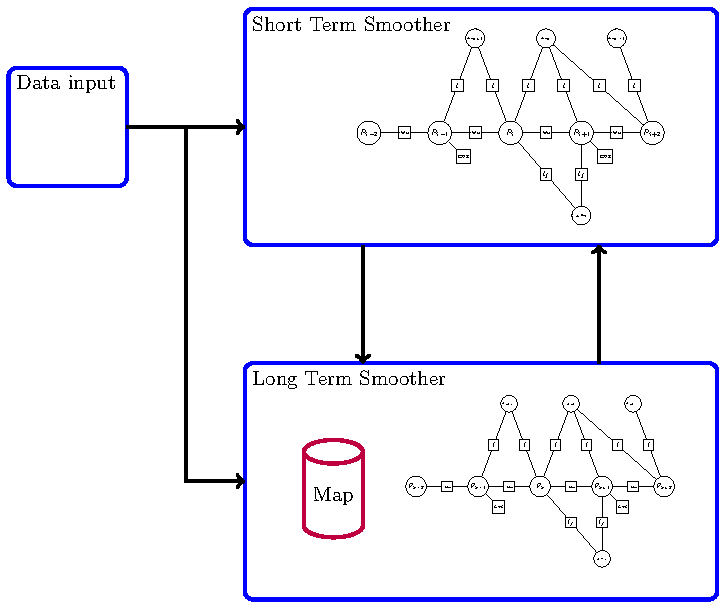
\includegraphics[width=0.99\textwidth]{TikZ_drawings/Simple_STS_and_LTS_diagram_2/Simple_STS_and_LTS_2.pdf}\\
\end{minipage}

\tiny <It would be a cool slide to explain the loosely-coupled approach that we aim at and could be moved to the beginning.>
\normalsize

% STS marginalizing old states
% LTS storing in a map, inputting landmarks into STS and doing loop closure.

\clearpage

\ETHslide
\section*{Work done so far}
%probably split it into two slides and show what is done
%Backbone of the localization framework
\begin{minipage}{0.4\textwidth}

\footnotesize
	 Short Term Smoother 
		\begin{itemize}
			\item[\ETHitem] building a full factor graph given sensor data
			\item[\ETHitem] estimating position and passing data to LTS (?)
		\end{itemize}
		
\footnotesize		
	 Long Term Smoother
		\begin{itemize}
		 	\item[\ETHitem] building a map with the input data	
		 	\item[\ETHitem] "translating" the map to a factor graph
		 	\item[\ETHitem] optimizing the factor graph and updating data in the map
		\end{itemize}
\end{minipage}
\hspace{0.2cm}
\begin{minipage}{0.59\textwidth}
	\centering
	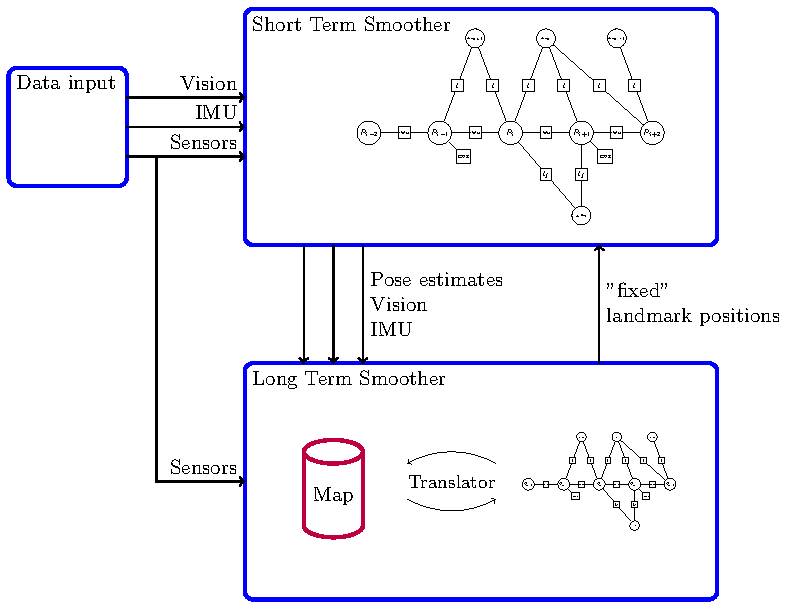
\includegraphics[width=0.99\textwidth]{TikZ_drawings/STS_and_LTS/STS_and_LTS.pdf}\\
\end{minipage}

		
		
\clearpage

\ETHslide
\section*{Current challenges}
\begin{itemize}
	\item[\ETHitem] Reading landmarks from the map and translating them into a factor graph
	\item[\ETHitem] Inserting "fixed" landmarks into STS
\end{itemize}

\begin{center}
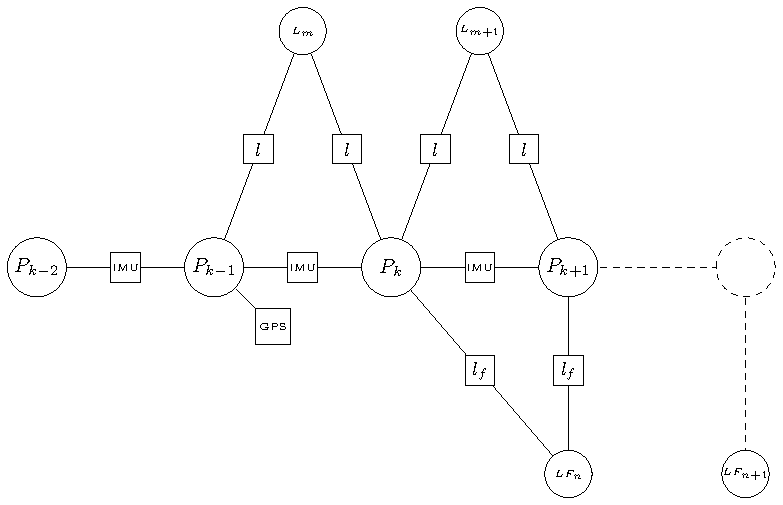
\includegraphics[width=0.6\textwidth]{TikZ_drawings/factor_graph_small/factor_graph.pdf}\\
\end{center}

\clearpage

\ETHslide
\section*{Future work}
\begin{itemize}
	\item[\ETHitem] 3-stage landmark initialization
	\begin{itemize}
		\item Stage 1: compute 3D landmark coordinate and initialize the feature as binary factor (state $x_k$ and $x_{k+1}$).
		% what is binary factor?
		\item Stage 2: formulate the feature re-projection factors connecting the 3D landmark state and pose.
		\item Stage 3: once uncertainty converges marginalize landmark state and switch back to binary factor formulation.
	\end{itemize}
 	\item[\ETHitem] Sliding-Window STS
	\begin{itemize}
		\item Reduce the STS problem to a sliding-window factor graph		
	\end{itemize} 	
\end{itemize}

\clearpage



\begin{comment}
References Slide
\ETHslide
\addcontentsline{toc}{section}{References}
\bibliographystyle{bibliography/IEEEtranN}
\tiny{
\bibliography{FILE}}
\clearpage
\end{comment}
\end{document}


